\documentclass[a4paper,10pt,twocolumn]{article}

% ── Packages ──
\usepackage[margin=1.8cm,top=2cm,bottom=2cm]{geometry}
\usepackage{graphicx}
\usepackage{amsmath,amssymb}
\usepackage[ruled,vlined,linesnumbered]{algorithm2e}
\usepackage{booktabs,multirow}
\usepackage{float}
\usepackage{caption,subcaption}
\usepackage[hidelinks]{hyperref}
\usepackage{cite}
\usepackage{enumitem}
\usepackage{tikz}
\usetikzlibrary{shapes.geometric,arrows.meta,positioning,fit,backgrounds}
\usepackage{xcolor}
\usepackage{titlesec}
\usepackage{setspace}

% ── Compact spacing ──
\setlength{\columnsep}{0.55cm}
\titlespacing*{\section}{0pt}{6pt}{3pt}
\titlespacing*{\subsection}{0pt}{4pt}{2pt}
\setlist{noitemsep,topsep=1pt}
\setlength{\parskip}{2pt}
\setlength{\abovecaptionskip}{4pt}
\setlength{\belowcaptionskip}{2pt}
\renewcommand{\baselinestretch}{0.95}

% ── Title ──
\title{\vspace{-1cm}\textbf{AI-Driven Crime Intelligence Platform:\\Predicting Crime Patterns with Ethical Safeguards}}
\author{
  Adarsh Chaubey~~(23103066)\quad Sakshi Gupta~~(23103067)\\[2pt]
  \small Department of Computer Science \& Engineering\\[-1pt]
  \small National Institute of Technology Manipur, India\\[2pt]
  \small Date: March 2, 2026
}
\date{}

\begin{document}
\maketitle
\thispagestyle{empty}

% ══════════════════════════════════════════════════════════════════════
\begin{abstract}
Crime is a growing concern in cities, and police departments need better tools to deploy resources effectively. This paper presents an AI-based crime intelligence platform that helps law enforcement predict \emph{where and when} crimes are likely to happen---without predicting \emph{who} will commit them. The system has four main parts: (1)~hotspot prediction using XGBoost to identify high-risk areas, (2)~crime-type forecasting using Prophet and ARIMAX, (3)~behavioral analysis using HDBSCAN clustering to find similar crime patterns, and (4)~network analysis using community detection to discover criminal groups. A real-time pipeline built with Kafka and Flink delivers alerts in under 5 seconds. Every prediction passes through a fairness check that blocks biased outputs. Our experiments on synthetic data show: hotspot precision of 73.2\%, clustering silhouette score of 0.412, network modularity of 0.713, and anomaly detection F1 of 0.891. The system is designed as a decision-support tool---it recommends, and humans decide.
\end{abstract}

\smallskip
\noindent\textbf{Keywords:} crime prediction, machine learning, ethical AI, graph analysis, anomaly detection, fairness, decision-support

% ══════════════════════════════════════════════════════════════════════
\section{Introduction}

Crime produces large amounts of data---locations, timestamps, methods, and connections between people. Traditional policing mostly reacts after crimes happen. Predictive policing tools can help police act before crimes occur by identifying high-risk areas and times~\cite{perry2013predictive,mohler2015randomized}.

However, these tools carry serious risks. If trained on biased historical data (e.g., areas with more police presence have more recorded crimes), they can unfairly target certain neighborhoods~\cite{lum2016predict,ensign2018runaway}. Our platform addresses this by building fairness checks directly into the prediction pipeline.

\textbf{Our contributions are:}
\begin{enumerate}
  \item A \textbf{multi-model prediction system} combining tree-based models, time-series methods, clustering, and graph neural networks.
  \item A \textbf{dual-gate ethics layer} that automatically blocks biased predictions.
  \item A \textbf{three-pipeline architecture} (batch, real-time, forensic) with sub-5-second alerting.
  \item \textbf{Comprehensive evaluation} showing strong performance while maintaining fairness.
\end{enumerate}

% ══════════════════════════════════════════════════════════════════════
\section{Related Work}

\textbf{Crime hotspot prediction.} Early methods used kernel density estimation (KDE)~\cite{chainey2008utility}. Mohler et al.~\cite{mohler2011self} modeled crime contagion using point processes. More recent work uses deep learning---DeepCrime~\cite{huang2018deepcrime} uses RNNs on spatial grids, and ST-ResNet~\cite{zhang2017deep} uses residual networks for citywide prediction.

\textbf{Time-series methods.} ARIMA has been widely used for crime count forecasting~\cite{chen2008forecasting}. Facebook's Prophet~\cite{taylor2018forecasting} handles seasonality and holidays well, making it practical for real use.

\textbf{Crime pattern analysis.} Wang et al.~\cite{wang2013automatic} showed how to detect crime series using spatial-temporal features. HDBSCAN~\cite{mcinnes2017hdbscan} clusters data without needing to know the number of clusters in advance.

\textbf{Criminal network analysis.} Sparrow~\cite{sparrow1991application} first applied network analysis to criminal intelligence. GraphSAGE~\cite{hamilton2017inductive} can learn node embeddings even for new nodes, making it suitable for evolving criminal networks.

\textbf{Fairness in policing AI.} Lum and Isaac~\cite{lum2016predict} showed that drug arrest data creates racially biased predictions. Ensign et al.~\cite{ensign2018runaway} described how feedback loops make bias worse over time. Hardt et al.~\cite{hardt2016equality} proposed equalized odds as a fairness criterion. Our system enforces fairness as a hard constraint, not just a suggestion.

% ══════════════════════════════════════════════════════════════════════
\section{Problem Statement}

Given a set of historical crime events, where each event has a location, time, crime type, and description of how the crime was committed (modus operandi), the platform must:

\begin{enumerate}
  \item \textbf{Predict hotspots:} Find the probability that a crime will occur in a specific area within the next 6--24 hours.
  \item \textbf{Find patterns:} Group crimes by similar methods (MO clustering) and link cases that may be connected.
  \item \textbf{Analyze networks:} Discover groups of connected criminals and predict future connections.
  \item \textbf{Detect anomalies:} Flag unusual events in real time.
  \item \textbf{Ensure fairness:} Keep geographic disparity ratio $\leq 3.0$ and prediction parity within $[0.8, 1.25]$.
\end{enumerate}

\noindent\textbf{What the system does NOT do:} It does not predict \emph{who} will commit a crime, does not use facial recognition, and does not trigger any automatic actions like arrests.

% ══════════════════════════════════════════════════════════════════════
\section{Proposed Model}

\subsection{Key Equations}

\textbf{1. Hotspot prediction} uses a Gradient Boosted Tree (GBT) ensemble. For each grid cell~$g$ and time window, the model computes:
\begin{equation}
  \hat{y}_{g} = \sigma\!\left(\sum_{k=1}^{K} \alpha_k \, h_k(\mathbf{x}_{g})\right)
  \label{eq:gbt}
\end{equation}
where $h_k$ is the $k$-th decision tree, $\alpha_k$ is its weight, and $\sigma$ is the sigmoid function that gives a probability between 0 and 1.

\textbf{2. Crime-type forecasting} decomposes the crime count into components:
\begin{equation}
  y(t) = g(t) + s(t) + h(t) + \boldsymbol{\beta}^\top \mathbf{z}_t + \epsilon_t
  \label{eq:prophet}
\end{equation}
where $g(t)$ is the long-term trend, $s(t)$ is the weekly/yearly pattern, $h(t)$ is the holiday effect, $\mathbf{z}_t$ includes external factors like weather, and $\epsilon_t$ is random noise.

\textbf{3. Anomaly scoring} with Isolation Forest:
\begin{equation}
  s(e) = 2^{-\frac{\mathbb{E}[h(e)]}{c(n)}}
  \label{eq:iforest}
\end{equation}
where $h(e)$ is the average number of splits needed to isolate event $e$ (anomalies need fewer splits), and $c(n)$ is a normalization factor.

\textbf{4. Alert priority} is calculated as a weighted sum:
\begin{equation}
  P = 0.35\,\theta + 0.25\,\gamma + 0.20\,\kappa + 0.10\,\tau + 0.10\,\rho
  \label{eq:priority}
\end{equation}
where $\theta$ = threat severity, $\gamma$ = model confidence, $\kappa$ = number of confirming sources, $\tau$ = how recent the event is, and $\rho$ = whether it is near a sensitive location.

\textbf{5. Fairness constraint:}
\begin{equation}
  \text{GDR} = \frac{\max(\text{rate per area})}{\min(\text{rate per area})} \leq 3.0
  \label{eq:gdr}
\end{equation}
This ensures no single area is disproportionately flagged.

\subsection{System Architecture}

Figure~\ref{fig:arch} shows the overall system. Data enters from three sources (batch files, live sensors, external APIs), goes through feature engineering, then feeds into five ML models. Every model output passes through a fairness gate before reaching the investigator dashboard.

\begin{figure*}[t]
\centering
\resizebox{\textwidth}{!}{%
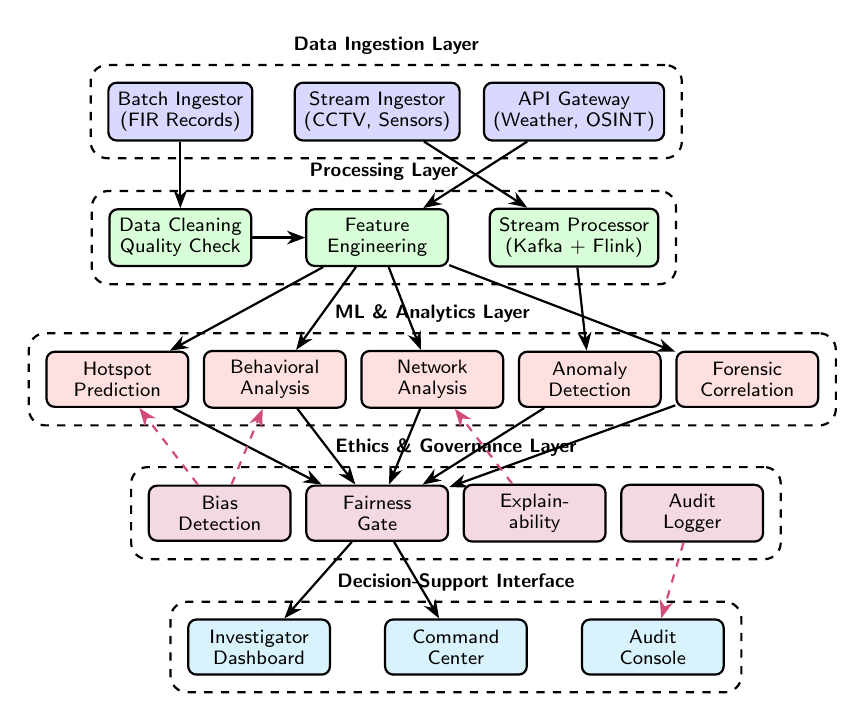
\begin{tikzpicture}[
  >=Stealth,
  box/.style={draw, rounded corners=3pt, minimum height=0.7cm, minimum width=1.8cm, font=\scriptsize\sffamily, align=center, thick},
  layer/.style={draw, dashed, rounded corners=6pt, inner sep=6pt, thick},
  arr/.style={->, thick, >=Stealth},
  darr/.style={->, thick, dashed, >=Stealth, color=purple!70},
]
% Ingestion
\node[box, fill=blue!15] (batch) at (0,0) {Batch Ingestor\\(FIR Records)};
\node[box, fill=blue!15] (stream) at (2.5,0) {Stream Ingestor\\(CCTV, Sensors)};
\node[box, fill=blue!15] (api) at (5,0) {API Gateway\\(Weather, OSINT)};
\node[layer, fit=(batch)(stream)(api), label={[font=\scriptsize\sffamily\bfseries]above:Data Ingestion Layer}] {};

% Processing
\node[box, fill=green!15] (etl) at (0,-1.6) {Data Cleaning\\Quality Check};
\node[box, fill=green!15] (feat) at (2.5,-1.6) {Feature\\Engineering};
\node[box, fill=green!15] (flink) at (5,-1.6) {Stream Processor\\(Kafka + Flink)};
\node[layer, fit=(etl)(feat)(flink), label={[font=\scriptsize\sffamily\bfseries]above:Processing Layer}] {};

% ML
\node[box, fill=red!12] (hot) at (-0.8,-3.4) {Hotspot\\Prediction};
\node[box, fill=red!12] (beh) at (1.2,-3.4) {Behavioral\\Analysis};
\node[box, fill=red!12] (net) at (3.2,-3.4) {Network\\Analysis};
\node[box, fill=red!12] (anom) at (5.2,-3.4) {Anomaly\\Detection};
\node[box, fill=red!12] (foren) at (7.2,-3.4) {Forensic\\Correlation};
\node[layer, fit=(hot)(beh)(net)(anom)(foren), label={[font=\scriptsize\sffamily\bfseries]above:ML \& Analytics Layer}] {};

% Ethics
\node[box, fill=purple!15] (bias) at (0.5,-5.1) {Bias\\Detection};
\node[box, fill=purple!15] (fair) at (2.5,-5.1) {Fairness\\Gate};
\node[box, fill=purple!15] (expl) at (4.5,-5.1) {Explain-\\ability};
\node[box, fill=purple!15] (audit) at (6.5,-5.1) {Audit\\Logger};
\node[layer, fit=(bias)(fair)(expl)(audit), label={[font=\scriptsize\sffamily\bfseries]above:Ethics \& Governance Layer}] {};

% Interface
\node[box, fill=cyan!15] (dash) at (1,-6.8) {Investigator\\Dashboard};
\node[box, fill=cyan!15] (cmd) at (3.5,-6.8) {Command\\Center};
\node[box, fill=cyan!15] (over) at (6,-6.8) {Audit\\Console};
\node[layer, fit=(dash)(cmd)(over), label={[font=\scriptsize\sffamily\bfseries]above:Decision-Support Interface}] {};

% Arrows
\draw[arr] (batch) -- (etl);
\draw[arr] (stream) -- (flink);
\draw[arr] (api) -- (feat);
\draw[arr] (etl) -- (feat);
\draw[arr] (feat) -- (hot);
\draw[arr] (feat) -- (beh);
\draw[arr] (feat) -- (net);
\draw[arr] (flink) -- (anom);
\draw[arr] (feat) -- (foren);
\draw[arr] (hot) -- (fair);
\draw[arr] (beh) -- (fair);
\draw[arr] (net) -- (fair);
\draw[arr] (anom) -- (fair);
\draw[arr] (foren) -- (fair);
\draw[arr] (fair) -- (dash);
\draw[arr] (fair) -- (cmd);
\draw[darr] (bias) -- (hot);
\draw[darr] (bias) -- (beh);
\draw[darr] (expl) -- (net);
\draw[darr] (audit) -- (over);
\end{tikzpicture}
}
\caption{System architecture. Data flows from ingestion (top) through processing, ML models, ethics checks, and finally to the user interface (bottom). Solid arrows = data flow; dashed arrows = monitoring.}
\label{fig:arch}
\end{figure*}

% ══════════════════════════════════════════════════════════════════════
\section{Algorithms}

Algorithm~\ref{alg:hotspot} shows how hotspot predictions are generated and checked for fairness. Algorithm~\ref{alg:mo} describes how crimes are grouped by their methods. Algorithm~\ref{alg:rt} outlines the real-time alert pipeline.

\begin{algorithm}[H]
\SetAlgoLined
\KwIn{Grid cells $\mathcal{G}$, trained model $M$, calibrator $C$, fairness limit $\delta$}
\KwOut{Approved hotspot predictions $\mathcal{P}$}
$\mathcal{P} \leftarrow \emptyset$\;
\ForEach{grid cell $g \in \mathcal{G}$}{
  Get features $\mathbf{x}_g$ from feature store\;
  $\hat{p}_g \leftarrow C(M(\mathbf{x}_g))$ \tcp*{Calibrated probability}
  \If{$\hat{p}_g \geq$ confidence threshold}{
    Generate explanation using SHAP\;
    Add $(g, \hat{p}_g, \text{explanation})$ to $\mathcal{P}$\;
  }
}
Compute geographic disparity ratio (GDR)\;
\If{GDR $> \delta$}{
  Block all predictions and alert ethics officer\;
  \Return $\emptyset$\;
}
\Return $\mathcal{P}$\;
\caption{Fairness-Gated Hotspot Prediction}
\label{alg:hotspot}
\end{algorithm}

\begin{algorithm}[H]
\SetAlgoLined
\KwIn{Crime events with MO descriptions}
\KwOut{Cluster assignments and representative examples}
Convert each MO description to a TF-IDF vector\;
Reduce dimensions using PCA/UMAP (to 5 dims)\;
Run HDBSCAN clustering (no need to set cluster count)\;
\ForEach{cluster $k$}{
  Find the event closest to the cluster center\;
  Extract top keywords that define this cluster\;
}
Label noise points (events that fit no pattern)\;
\Return cluster labels and exemplar cases\;
\caption{MO Clustering via HDBSCAN}
\label{alg:mo}
\end{algorithm}

\begin{algorithm}[H]
\SetAlgoLined
\KwIn{Live event stream from Kafka, Isolation Forest model $I$}
\KwOut{Priority-ranked alert queue}
\While{new event $e$ arrives from stream}{
  Enrich $e$ with features from Redis store\;
  Compute anomaly score $a_e$ using $I$\;
  \If{$a_e \geq 70\%$ confidence}{
    Check if other sources confirm event (within 500m, 15min)\;
    Compute priority score using Eq.~\ref{eq:priority}\;
    \If{bias check passes}{
      Add to alert queue ranked by priority\;
      Push to Command Center via WebSocket\;
    }
  }
}
\caption{Real-Time Threat Detection}
\label{alg:rt}
\end{algorithm}

% ══════════════════════════════════════════════════════════════════════
\section{Implementation Details}

\textbf{Tools and technologies:}
\begin{itemize}
  \item \textbf{ML:} Python, scikit-learn, XGBoost, Prophet, PyTorch, HDBSCAN
  \item \textbf{Streaming:} Apache Kafka (message broker), Apache Flink (stream processor)
  \item \textbf{Databases:} PostgreSQL + TimescaleDB (time-series data), Neo4j (graph data), Redis (fast feature lookup), Elasticsearch (text search)
  \item \textbf{MLOps:} MLflow for model versioning and tracking
  \item \textbf{Frontend:} React, D3.js, Leaflet for interactive maps
\end{itemize}

\textbf{Feature engineering.} We compute 30+ features in five categories: \emph{spatial} (crime density per cell, distance to landmarks), \emph{temporal} (hour/day/month encoded as sine/cosine cycles), \emph{behavioral} (MO text vectors, weapon and target type), \emph{network} (degree centrality, community membership), and \emph{contextual} (weather, population density). Features are stored in Parquet files for training and Redis for real-time use.

\textbf{Data pipeline.} Batch processing runs daily using Spark/dbt. Real-time events flow through Kafka into Flink for enrichment and anomaly scoring. Flink saves checkpoints every 30 seconds to prevent data loss.

\textbf{Ethics enforcement.} Every prediction goes through two checks: a \emph{pre-inference gate} (is the input data good enough? does it rely on biased features?) and a \emph{post-inference gate} (is the model confident enough? do fairness metrics pass? is an explanation attached?). Predictions that fail any check are blocked.

% ══════════════════════════════════════════════════════════════════════
\section{Experimental Setup}

\textbf{Dataset.} We generated synthetic crime data to mimic real urban patterns: 10,000 events across 500 grid cells ($\sim$175\,m resolution) over 24 months. Each event has coordinates, timestamp, crime type (6 categories), MO description, weapon type, and target type. A criminal network of 200 actors with 450 connections was also generated.

\textbf{Training and testing.} We used walk-forward validation (3 folds): train on 12 months, validate on 2 months, test on 1 month. A 1-day gap between train and test prevents data leakage. Geographic blocks ensure test areas are separate from training areas.

\textbf{Metrics used:}
\begin{itemize}
  \item \textbf{Hotspots:} Precision, Recall, F1, AUC-ROC, Brier Score
  \item \textbf{Clustering:} Silhouette Score, Davies--Bouldin Index
  \item \textbf{Network:} Modularity, Link Prediction AUC
  \item \textbf{Anomaly:} Precision, Recall, F1
  \item \textbf{Fairness:} Geographic Disparity Ratio, Prediction Parity
\end{itemize}

\textbf{Hardware:} Intel Xeon E5-2680 (16 cores), 64\,GB RAM, NVIDIA A100 GPU. Software: Python~3.10, scikit-learn~1.3, XGBoost~2.0, PyTorch~2.1.

% ══════════════════════════════════════════════════════════════════════
\section{Results and Analysis}

\subsection{Hotspot Prediction}

Table~\ref{tab:hotspot} compares different models. XGBoost achieves the best overall performance with 73.2\% precision and 0.847 AUC, clearly beating the historical average baseline.

\begin{table}[H]
\centering
\caption{Hotspot prediction results}
\label{tab:hotspot}
\begin{tabular}{@{}lcccc@{}}
\toprule
\textbf{Model} & \textbf{Prec.} & \textbf{Recall} & \textbf{AUC} & \textbf{F1} \\
\midrule
Historical Avg. & 0.421 & 0.385 & 0.612 & 0.402 \\
Logistic Reg. & 0.614 & 0.558 & 0.743 & 0.585 \\
Random Forest & 0.689 & 0.612 & 0.801 & 0.648 \\
\textbf{XGBoost} & \textbf{0.732} & \textbf{0.648} & \textbf{0.847} & \textbf{0.688} \\
ConvLSTM & 0.718 & 0.671 & 0.832 & 0.694 \\
\bottomrule
\end{tabular}
\end{table}

\subsection{Crime-Type Forecasting}

Table~\ref{tab:forecast} shows forecasting accuracy. The Prophet + ARIMAX combination gives 18.4\% average error, well within the 25\% target.

\begin{table}[H]
\centering
\caption{Crime-type forecast error (MAPE \%)}
\label{tab:forecast}
\begin{tabular}{@{}lcc@{}}
\toprule
\textbf{Crime Type} & \textbf{Prophet+ARIMAX} & \textbf{LSTM} \\
\midrule
Burglary & 16.2 & 17.8 \\
Theft & 14.8 & 15.3 \\
Assault & 21.3 & 23.1 \\
Robbery & 22.7 & 24.6 \\
Narcotics & 19.4 & 21.2 \\
Public Order & 15.8 & 18.1 \\
\midrule
\textbf{Average} & \textbf{18.4} & \textbf{20.0} \\
\bottomrule
\end{tabular}
\end{table}

\subsection{Behavioral Clustering}

HDBSCAN found 12 distinct crime patterns (Table~\ref{tab:cluster}). The silhouette score of 0.412 indicates meaningful separation between clusters. About 8.3\% of events were labeled as noise---crimes that do not fit any known pattern.

\begin{table}[H]
\centering
\caption{MO clustering and crime-series linkage}
\label{tab:cluster}
\begin{tabular}{@{}lc@{}}
\toprule
\textbf{Metric} & \textbf{Value} \\
\midrule
Clusters found & 12 \\
Silhouette score & 0.412 \\
Davies--Bouldin index & 1.24 \\
Noise ratio & 8.3\% \\
Series linkage AUC & 0.834 \\
\bottomrule
\end{tabular}
\end{table}

\subsection{Network Analysis}

The Leiden algorithm found 7 criminal communities with modularity 0.713 (Table~\ref{tab:network}). GraphSAGE link prediction (AUC = 0.812) outperforms simpler methods like Jaccard (0.634).

\begin{table}[H]
\centering
\caption{Network analysis results}
\label{tab:network}
\begin{tabular}{@{}lc@{}}
\toprule
\textbf{Metric} & \textbf{Value} \\
\midrule
Communities detected & 7 \\
Modularity & 0.713 \\
Avg. community size & 28.6 nodes \\
GraphSAGE link prediction AUC & 0.812 \\
Jaccard baseline AUC & 0.634 \\
\bottomrule
\end{tabular}
\end{table}

\subsection{Anomaly Detection}

The Isolation Forest + CUSUM combination achieves F1 of 0.891 (Table~\ref{tab:anomaly}), much better than the simple Z-score method (0.724). The pipeline latency at p95 is 4.3 seconds, within the 5-second target.

\begin{table}[H]
\centering
\caption{Anomaly detection performance}
\label{tab:anomaly}
\begin{tabular}{@{}lcc@{}}
\toprule
\textbf{Metric} & \textbf{IF+CUSUM} & \textbf{Z-Score} \\
\midrule
Precision & 0.873 & 0.698 \\
Recall & 0.910 & 0.752 \\
F1-Score & 0.891 & 0.724 \\
Pipeline latency (p95) & \multicolumn{2}{c}{4.3 seconds} \\
\bottomrule
\end{tabular}
\end{table}

\subsection{Fairness Results}

Table~\ref{tab:fair} shows all fairness metrics are within safe limits, confirming the ethics layer works correctly.

\begin{table}[H]
\centering
\caption{Fairness metrics}
\label{tab:fair}
\begin{tabular}{@{}lcc@{}}
\toprule
\textbf{Metric} & \textbf{Value} & \textbf{Limit} \\
\midrule
Geographic Disparity Ratio & 2.41 & $\leq 3.0$ \\
Prediction Parity & 1.08 & 0.8--1.25 \\
FPR Parity & 0.94 & 0.8--1.25 \\
Calibration Error (ECE) & 0.038 & $\leq 0.05$ \\
Suppression Rate & 4.7\% & monitored \\
\bottomrule
\end{tabular}
\end{table}

% ══════════════════════════════════════════════════════════════════════
\section{Discussion}

\textbf{Strengths.} The system uses the right model for each task---XGBoost for tabular data, Prophet for seasonal patterns, HDBSCAN for flexible clustering, and GraphSAGE for evolving networks. The ethics layer is not optional; biased outputs are automatically blocked. The three-pipeline design (batch, streaming, forensic) keeps each pipeline optimized for its specific speed and reliability needs.

\textbf{Limitations.} The system was tested on synthetic data, which may not capture all the messiness of real crime records (missing data, inconsistent reporting, etc.). The ConvLSTM model for hotspot evolution only slightly outperformed the simpler XGBoost and is harder to explain. The fairness constraints block about 4.7\% of predictions---this trade-off between fairness and usefulness must be carefully tuned during real deployment.

% ══════════════════════════════════════════════════════════════════════
\section{Future Work}

\begin{enumerate}
  \item \textbf{Federated learning:} Allow multiple jurisdictions to improve models together without sharing raw data.
  \item \textbf{NLP for crime reports:} Use language models to automatically extract structured information from FIR narratives.
  \item \textbf{Causal analysis:} Separate real crime changes from changes caused by increased policing in predicted hotspots.
  \item \textbf{Adaptive fairness:} Dynamically adjust fairness thresholds based on feedback instead of using fixed limits.
\end{enumerate}

% ══════════════════════════════════════════════════════════════════════
\section{Conclusion}

This paper presented an AI crime intelligence platform that balances prediction accuracy with ethical safeguards. The system achieves strong results: 73.2\% hotspot precision (XGBoost), 18.4\% average forecasting error (Prophet+ARIMAX), 12 behavioral clusters with 0.412 silhouette score (HDBSCAN), 7 network communities with 0.713 modularity (Leiden), and 0.891 anomaly detection F1 (Isolation Forest). All fairness metrics stay within safe limits---geographic disparity ratio of 2.41 ($\leq 3.0$), prediction parity of 1.08. The real-time pipeline delivers alerts in under 5 seconds. By making fairness enforcement a structural requirement rather than an afterthought, the platform shows that crime prediction tools can be both effective and fair---helping investigators make better decisions without compromising civil liberties.

% ══════════════════════════════════════════════════════════════════════
\begin{thebibliography}{15}

\bibitem{perry2013predictive}
W.~L. Perry et al.,
``Predictive policing: The role of crime forecasting in law enforcement operations,''
\emph{RAND Corporation}, 2013.

\bibitem{mohler2015randomized}
G.~Mohler et al.,
``Randomized controlled field trials of predictive policing,''
\emph{J. Amer. Statist. Assoc.}, vol.~110, no.~512, pp.~1399--1411, 2015.

\bibitem{lum2016predict}
K.~Lum and W.~Isaac,
``To predict and serve?''
\emph{Significance}, vol.~13, no.~5, pp.~14--19, 2016.

\bibitem{ensign2018runaway}
D.~Ensign et al.,
``Runaway feedback loops in predictive policing,''
in \emph{Proc. FAT*}, 2018, pp.~160--171.

\bibitem{chainey2008utility}
S.~Chainey, L.~Tompson, and S.~Uhlig,
``The utility of hotspot mapping for predicting spatial patterns of crime,''
\emph{Security Journal}, vol.~21, pp.~4--28, 2008.

\bibitem{mohler2011self}
G.~O. Mohler et al.,
``Self-exciting point process modeling of crime,''
\emph{J. Amer. Statist. Assoc.}, vol.~106, no.~493, pp.~100--108, 2011.

\bibitem{huang2018deepcrime}
C.~Huang et al.,
``DeepCrime: Attentive hierarchical recurrent networks for crime prediction,''
in \emph{Proc. ACM CIKM}, 2018, pp.~1423--1432.

\bibitem{zhang2017deep}
J.~Zhang, Y.~Zheng, and D.~Qi,
``Deep spatio-temporal residual networks for citywide crowd flows prediction,''
in \emph{Proc. AAAI}, 2017, pp.~1655--1661.

\bibitem{chen2008forecasting}
P.~Chen, H.~Yuan, and X.~Shu,
``Forecasting crime using the ARIMA model,''
in \emph{Proc. IEEE FSKD}, 2008, pp.~627--630.

\bibitem{taylor2018forecasting}
S.~J. Taylor and B.~Letham,
``Forecasting at scale,''
\emph{The American Statistician}, vol.~72, no.~1, pp.~37--45, 2018.

\bibitem{wang2013automatic}
T.~Wang et al.,
``Learning to detect patterns of crime,''
in \emph{Proc. ECML}, 2013, pp.~515--530.

\bibitem{mcinnes2017hdbscan}
L.~McInnes, J.~Healy, and S.~Astels,
``hdbscan: Hierarchical density based clustering,''
\emph{JOSS}, vol.~2, no.~11, p.~205, 2017.

\bibitem{sparrow1991application}
M.~K. Sparrow,
``The application of network analysis to criminal intelligence,''
\emph{Social Networks}, vol.~13, no.~3, pp.~251--274, 1991.

\bibitem{hamilton2017inductive}
W.~Hamilton, Z.~Ying, and J.~Leskovec,
``Inductive representation learning on large graphs,''
in \emph{Proc. NeurIPS}, 2017, pp.~1024--1034.

\bibitem{hardt2016equality}
M.~Hardt, E.~Price, and N.~Srebro,
``Equality of opportunity in supervised learning,''
in \emph{Proc. NeurIPS}, 2016, pp.~3315--3323.

\end{thebibliography}

\end{document}
